\documentclass{report}
    \title{50003 - Models of Computation - Lecture 6}
    \author{Oliver Killane}
    \date{29/10/21}

%===========================COMMON FORMAT & COMMANDS===========================
% This file contains commands and format to be used by every module, and is 
% included in all files.
%===============================================================================

%====================================IMPORTS====================================
\usepackage[a4paper, total={6in, 8in}]{geometry}
\usepackage{graphicx, amssymb, amsfonts, amsmath, xcolor, listings, tcolorbox, multirow, hyperref}
%===============================================================================

%====================================IMAGES=====================================
\graphicspath{{image/}}

% \centerimage{options}{image}
\newcommand{\centerimage}[2]{\begin{center}
    \includegraphics[#1]{#2}
\end{center}}
%===============================================================================

%=================================CODE LISTINGS=================================
\definecolor{codebackdrop}{gray}{0.9}
\definecolor{commentgreen}{rgb}{0,0.6,0}
\lstset{
    inputpath=code, 
    commentstyle=\color{commentgreen},
    keywordstyle=\color{blue}, 
    backgroundcolor=\color{codebackdrop}, 
    basicstyle=\footnotesize,
    frame=single,
    numbers=left,
    stepnumber=1,
    showstringspaces=false,
    breaklines=true,
    postbreak=\mbox{\textcolor{red}{$\hookrightarrow$}\space}
}

% Create a code listing for a single line
% \codeline{language}{line}{file}
\newcommand{\codeline}[3]{\lstinputlisting[language=#1, firstline = #2, lastline = #2]{#3}}

% Create a code listing for a given language & file
% \codelist{language}{file}
\newcommand{\codelist}[2]{\lstinputlisting[language=#1]{#2}}
%===============================================================================

%================================TEXT STRUCTURES================================
% Marka a word as bold
% \keyword{important word}
\newcommand{\keyword}[1]{\textbf{#1}}

% Creates a section in italics
% \question{question in italics}
\newcommand{\question}[1]{\textit{#1} \\ }

% Creates a box with title for side notes.
% \sidenote{title}{contents}
\newcommand{\sidenote}[2]{\begin{tcolorbox}[title=#1]#2\end{tcolorbox}}

% Creates an item in an itemize or enumerate, with a paragraph after
% \begin{itemize}
%     \bullpara{title}{contents}
% \end{itemize}
\newcommand{\bullpara}[2]{\item \textbf{#1} \ #2}

% Creates a compact list (very small gaps between items)
% \compitem{
%     \item item 1
%     \item item 2
%     \item ...
% }
\newcommand{\compitem}[1]{\begin{itemize}\setlength\itemsep{-0.5em}#1\end{itemize}}

% Creates a link to the lecture for use at the start of the notes document
\newcommand{\lectlink}[1]{\sidenote{Lecture Recording}{
    Lecture recording is available \href{#1}{here}
}}
%===============================================================================


%================================CONFIGURATIONS================================
\newcommand{\config}[2]{\langle #1, #2 \rangle}
%==============================================================================

%==============================BIG STEP SEMANTICS==============================
\newcommand{\bigstep}[4]{\text{(#1)}\dfrac{#2}{#3 \Downarrow #4}}
\newcommand{\bigstepdef}[5]{\bigstep{#1}{#2}{#3}{#4} \ #5}
%==============================================================================

%=============================SMALL STEP SEMANTICS=============================
\newcommand{\smallstep}[4]{\text{(#1)}\dfrac{#2}{#3 \to #4}}
\newcommand{\smallstepdef}[5]{\smallstep{#1}{#2}{#3}{#4} \ #5}
%==============================================================================

\newcommand{\whilest}[3]{\text{(#1)}\dfrac{#2}{#3}}
\newcommand{\whilestdef}[4]{\whilest{#1}{#2}{#3} \ #4}
%==============================================================================

%===================================COMMANDS===================================
\newcommand{\while}[2]{\text{while } #1 \text{ do } #2}
\newcommand{\cond}[3]{\text{if } #1 \text{ then } #2 \text{ else } #3}
\newcommand{\doret}[2]{\text{do } #1 \text{ return } #2}

\newcommand{\instrlabel}[1]{\text{\textcolor{teal}{$L_{#1}$}}}
\newcommand{\reglabel}[1]{\text{\textcolor{orange}{$R_{#1}$}}}
\newcommand{\regtemp}[1]{\text{\textcolor{orange}{$#1$}}}
\newcommand{\instr}[2]{\instrlabel{#1} : & #2 \\}
\newcommand{\dec}[3]{\reglabel{#1}^- \to \instrlabel{#2}, \instrlabel{#3}}
\newcommand{\inc}[2]{\reglabel{#1}^+ \to \instrlabel{#2}}
\newcommand{\halt}{\text{\textcolor{red}{\textbf{HALT}}}}

\newcommand{\lambapp}[2]{#1 \ #2}
\newcommand{\lambappb}[2]{(#1) \ (#2)}
\newcommand{\lambfun}[2]{\lambda #1 \ . \ #2}

\makeatletter
\newcommand{\lambarg}[1]{%
	#1 \checknextarglambarg}
\newcommand{\checknextarglambarg}{\@ifnextchar\bgroup{\gobblenextarglambarg}{}}
\newcommand{\gobblenextarglambarg}[1]{ \ #1 \@ifnextchar\bgroup{\gobblenextarglambarg}{}}

\newcommand{\chnum}[1]{\underline{#1}}
% Variable argument regconfig \regconfig{label no}{reg val}{reg val}...
\makeatletter
\newcommand{\regconfig}[2]{%
	$#1$ & $#2$\checknextarg}
\newcommand{\checknextarg}{\@ifnextchar\bgroup{\gobblenextarg}{\\}}
\newcommand{\gobblenextarg}[1]{ & $#1$\@ifnextchar\bgroup{\gobblenextarg}{\\}}
%==============================================================================

\begin{document}
    \maketitle
    \lectlink{https://imperial.cloud.panopto.eu/Panopto/Pages/Viewer.aspx?id=d355a5c2-e54d-4d4a-8088-add001358315}

    \section*{Definition by Induction for SimpleExp}
        To define a function on all expressions in \keyword{SimpleExp}:
        \compitem{
            \item define $f(n)$ directly, for each number $n$.
            \item define $f(E_1 + E_2)$ in terms of $f(E_1)$ and $f(E_2)$.
            \item define $f(E_1 \times E_2)$ in terms of $f(E_1)$ and $f(E_2)$.
        }
        For example, we can do this with $den$:
        \[den(E = n \leftrightarrow E \Downarrow n\]

    \section*{Evaluation}
        \subsection*{Many Steps of Evaluation}
            Given $\to$ we can define a new relation $\to^*$ as:
            \[E \to^* E' \leftrightarrow (E = E' \lor E \to E_1 \to E_2 \to \dots \to E_k \to E')\]
            For expressions, the final answer is $n$ if $E \to^* n$.
        \subsection*{Multi-Step Reductions}
            The relation $E \to^n E'$ is defined using mathematics induction by:
            \begin{itemize}
                \bullpara{Base Case}{
                    \\ $E \to^0 E$ for all $E \in SimpleExp$
                }
                \bullpara{Inductive Case}{
                    \\ For every $E,E' \in SimpleExp$, $E \to^{k+1}E'$ if and only if there is some $E''$ such that:
                    \[E \to^k E'' \land E'' \to E'\]
                }
                \bullpara{Definition}{
                    \\ $\to^*$ - there are some number of steps to evaluate to $E'$.
                    \[E \to^* E' \Leftrightarrow \exists n.[E \to^n E']\]
                }
            \end{itemize}
        \subsection*{Properties of $\to$}
            \begin{itemize}
                \bullpara{Determinacy}{ If $E \to E_1$ and $E \to E_2$ then $E_1 = E_2$.}
                \bullpara{Confluence}{If $E \to^* E_1$ and $E \to^*E_2$ then there exists $E'$ such that $E_1 \to^* E'$ and $E_2 \to^* E'$.}
                \bullpara{Unique answer}{If $E \to^* n_1$ and $E \to^* n_2$ then $N_1 = n_2$.}
                \bullpara{Normal Forms}{Normal form is numbers ($\mathbb{N}$) for any $E$, $E = n$ or $E \to E'$ for some $E'$.}
                \bullpara{Normalisation}{No infinite sequences of expressions $E_1,E_2,E_3, \dots$ such that for all $i \in \mathbb{N}$ $E_1 \to E_{i+1}$ (Every path goes to a normal form).}
            \end{itemize}

        \subsection*{Confluence of Small Step}
            We can prove a lemma expressing confluence:
            \[L_1 : \forall n \in \mathbb{N} . \forall E, E_1, E_2 \in SimpleExp . [E \to^n E_1 \land E \to^* E_2 \Rightarrow \exists E' \in SimpleExp . [E_1 \to^* E' \land E_2 \to^* E']]\]
            \subsubsection*{Lemma $\Rightarrow$ Confluence}
                Confluence is: $\forall E, E_1, E_2 \in SimpleExp . [E \to^* E_1 \land E \to^* E_2 \Rightarrow \exists E' \in SimpleExp . [E_1 \to^* E' \land E_2 \to^* E']]$
                From lemma $L_1$
                \begin{center}
                    \begin{tabular}{l l l}
                        (1) & Take some arbitrary $E, E_1, E_2 \in SimpleExp$, assume confluence holds. & (Initial Setup) \\
                        (2) & $E \to^* E_1$ & (By Confluence) \\
                        (3) & $\exists n \in \mathbb{N} .[E \to^n E_1]$ & (By 2 \& definition of $\to^*$) \\
                        (4) & Hence $L_1$ & (By 3) \\
                    \end{tabular}
                \end{center}
        \subsection*{Determinacy of Small Step}
            We create a property $P$:
            \[P(E) \overset{def}{=} \forall E_1,E_2 \in SimpleExp .[E \to E_1 \land E \to E_2 \Rightarrow E_1 = E_2] \]
            There are 3 rules that apply:
            \[\begin{matrix}
                \whilestdef{A}{}{n_1 + n_2 \to n}{n = n_1 + n_2} & \whilestdef{B}{E \to E'}{n + E \to n + E'}{} & \whilestdef{C}{E_1 \to E_1'}{E_1 + E_2 \to E_1' + E_2}{}
            \end{matrix}\]
            \subsubsection*{Base Case}
                Take arbitrary $n \in \mathbb{N}$ and $E_1,E_2 \in SimpleExp$ such that $n \to E_1 \land n \to E_2$ to show $E_1 = E_2$.
                \begin{center}
                    \begin{tabular}{l l l}
                        (1) & $n \not\to$ & (By inversion on A,B \& C) \\
                        (2) & $\neg (n \to E_1)$ & (By 1) \\
                        (3) & $\neg (n \to E_1 \land n \to E_2)$ & (By 2) \\
                        (4) & $E \to E_1 \land E \to E_2 \Rightarrow E_1 = E_2$ & (By 3) \\
                    \end{tabular}
                \end{center}
                Hence $P(n)$
            \subsubsection*{Inductive Step}
                Take arbitrary $E, E_1,E_2$ such that $E = E_1 + E_2$
                \\ Inductive Hypothesis:
                \[IH_1 = P(E_1)\]
                \[IH_2 = P(E_2)\]
                Assume there exists $E_3, E_4 \in SimpleExp$ such that $E_1 + E_2 \to E_3$ and $E_1 + E_2 \to E_4$.
                \\ To show $E_2 = E_4$.
                \\
                \\ From inversion on A, B \& C there are 3 cases to consider:
                \\ \textbf{For A:}
                \begin{center}
                    \begin{tabular}{l l l}
                        (1) & There exists $n_1, n_2 \in \mathbb{N}$ such that $E_1 = n_1$ and $E_2 = n_2$ & (By case A) \\
                        (3) & $E_3 = n_1 + n_2$ & (By 1, A) \\
                        (4) & $E_4 = n_1 + n_2$ & (By 1, A) \\
                        (5) & $E_3 = E_4$ & (By 3 \& 4) \\
                    \end{tabular}
                \end{center}
                \textbf{For B:}
                \begin{center}
                    \begin{tabular}{l l l}
                        (1) & There exists $n \in \mathbb{N}$ such that $E_1 = n$ & (By case B) \\
                        (2) & There exists $E' \in SimpleExp$ such that $E_2 \to E'$ & (By case B) \\
                        (3) & $E_3 = n + E'$ & (By case B) \\
                        (4) & There exists $E'' \in SimpleExp$ such that $E_2 \to E''$ & (By case B) \\
                        (5) & $E_4 = n + E''$ & (By case B) \\
                        (6) & $E' = E''$ & (By $IH_2$) \\
                        (7) & $E_3 = E_4$ & (By 3,5 \& 6) \\
                    \end{tabular}
                \end{center}
                \textbf{For C:}
                \begin{center}
                    \begin{tabular}{l l l}
                        (1) & There exists $E' \in SimpleExp$ such that $E_1 \to E'$ & (By case C) \\
                        (2) & There exists $E'' \in SimpleExp$ such that $E_1 \to E''$ & (By case C) \\
                        (3) & $E_3 = E' + E_2$ & (By case C) \\
                        (4) & $E_4 = E'' + E_2$ & (By case C) \\
                        (5) & $E' = E''$ & (By $IH_1$) \\
                        (6) & $E_3 = E_4$ & (By 3,4 \& 5)
                    \end{tabular}
                \end{center}
            (If $E$ reduces to $E_1$ in $n$ steps, and to $E_2$ in some number of steps, then there must be some $E'$ that $E_1$ and $E_2$ reduce to.)
            \subsubsection*{Base Case}
                The base cases has $n=0$. Hence $E = E_1$, and hence $E_1 \to^* E_2$ and $E_1 \to^* E'$
                \begin{center}
                    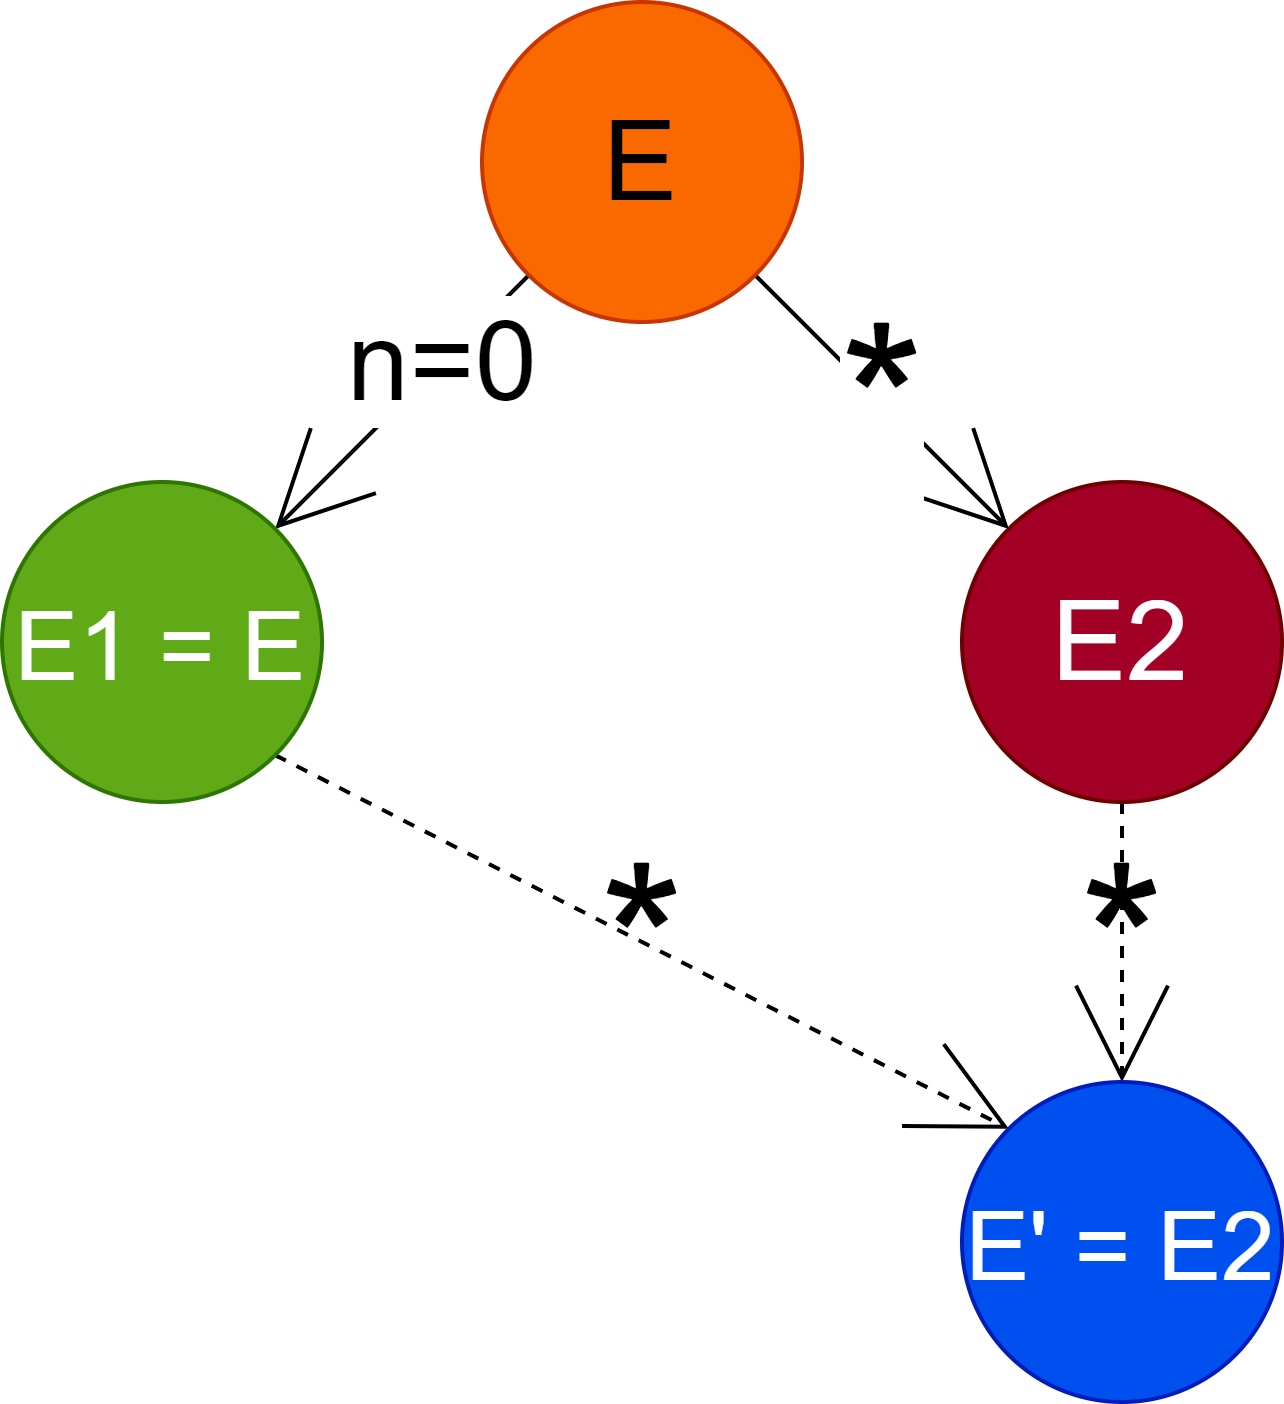
\includegraphics[scale=0.1]{confluence base case.png}
                \end{center}
            \subsubsection*{Inductive Case}
                Next we assume confluence for up to $k$ steps, and attempt to prove for $k+1$ steps.
                \begin{center}
                    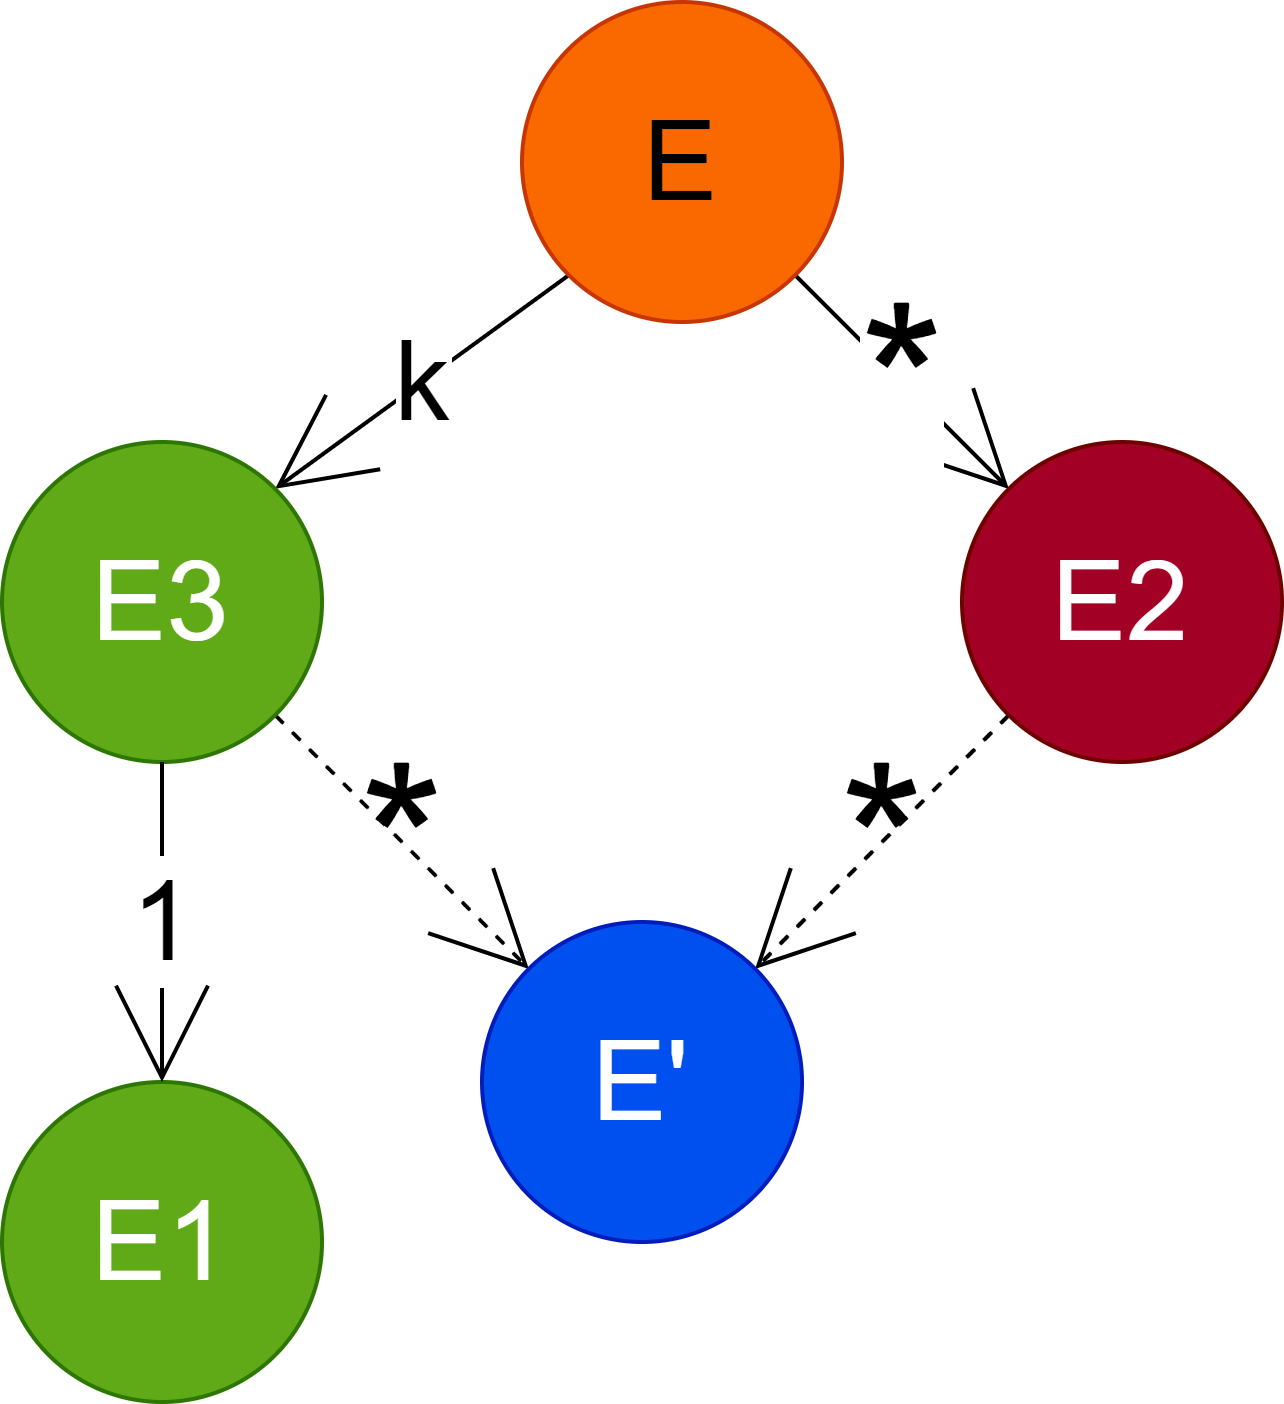
\includegraphics[scale=0.1]{confluence inductive case.png}
                \end{center}
                We have two cases:
                \\ \textbf{Case 1:} $E_3 = E'$, this is easy as $E_2 \to^* E' \to^0 E3 \to^1 E1$.
                \begin{center}
                    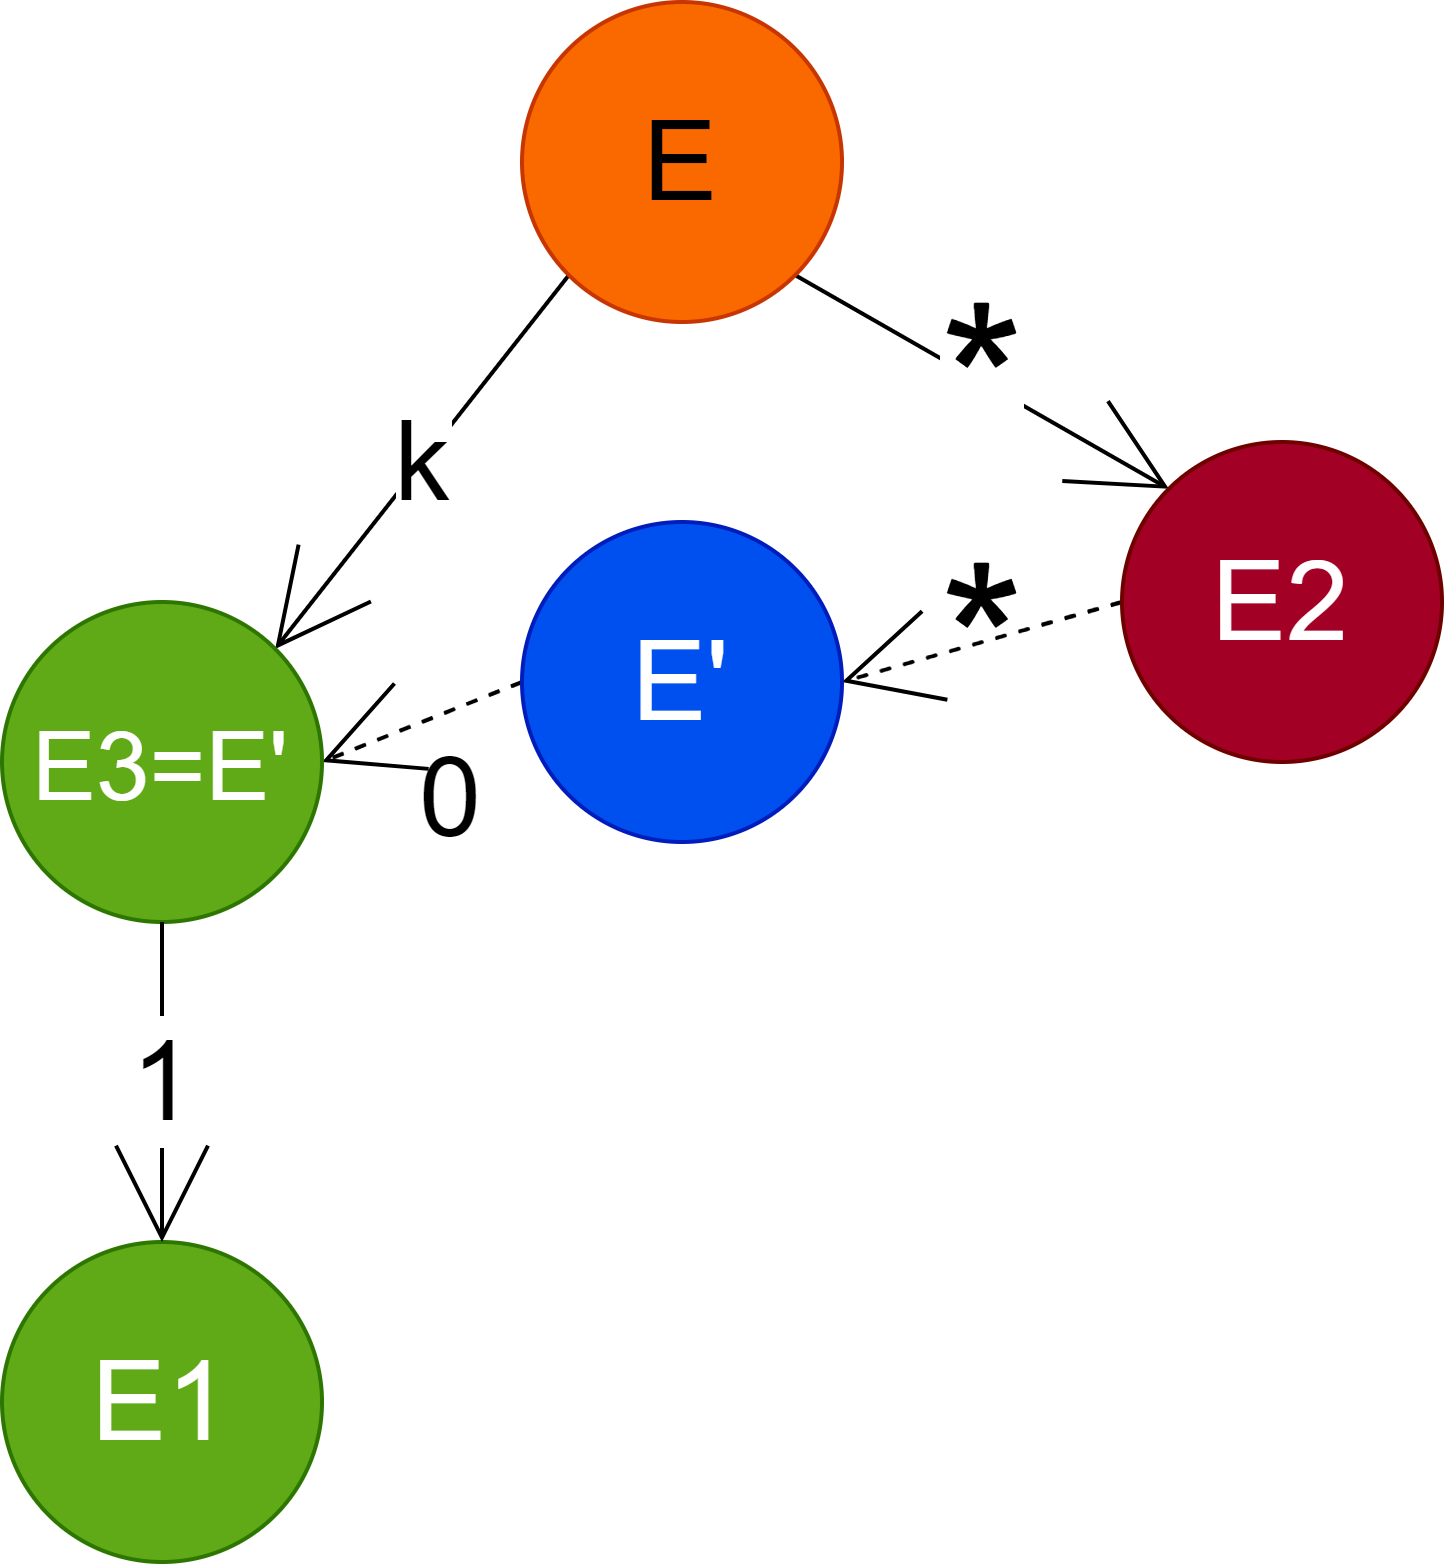
\includegraphics[scale=0.1]{confluence inductive case A.png}
                \end{center}
                \textbf{Case 2:} $E_3 \to^1 E'' \to^* E'$, in this case as $E_3 \to^1 E1$ we know by determinacy that $E'' = E_1$ and hence $E_1 \to^* E'$.
                \begin{center}
                    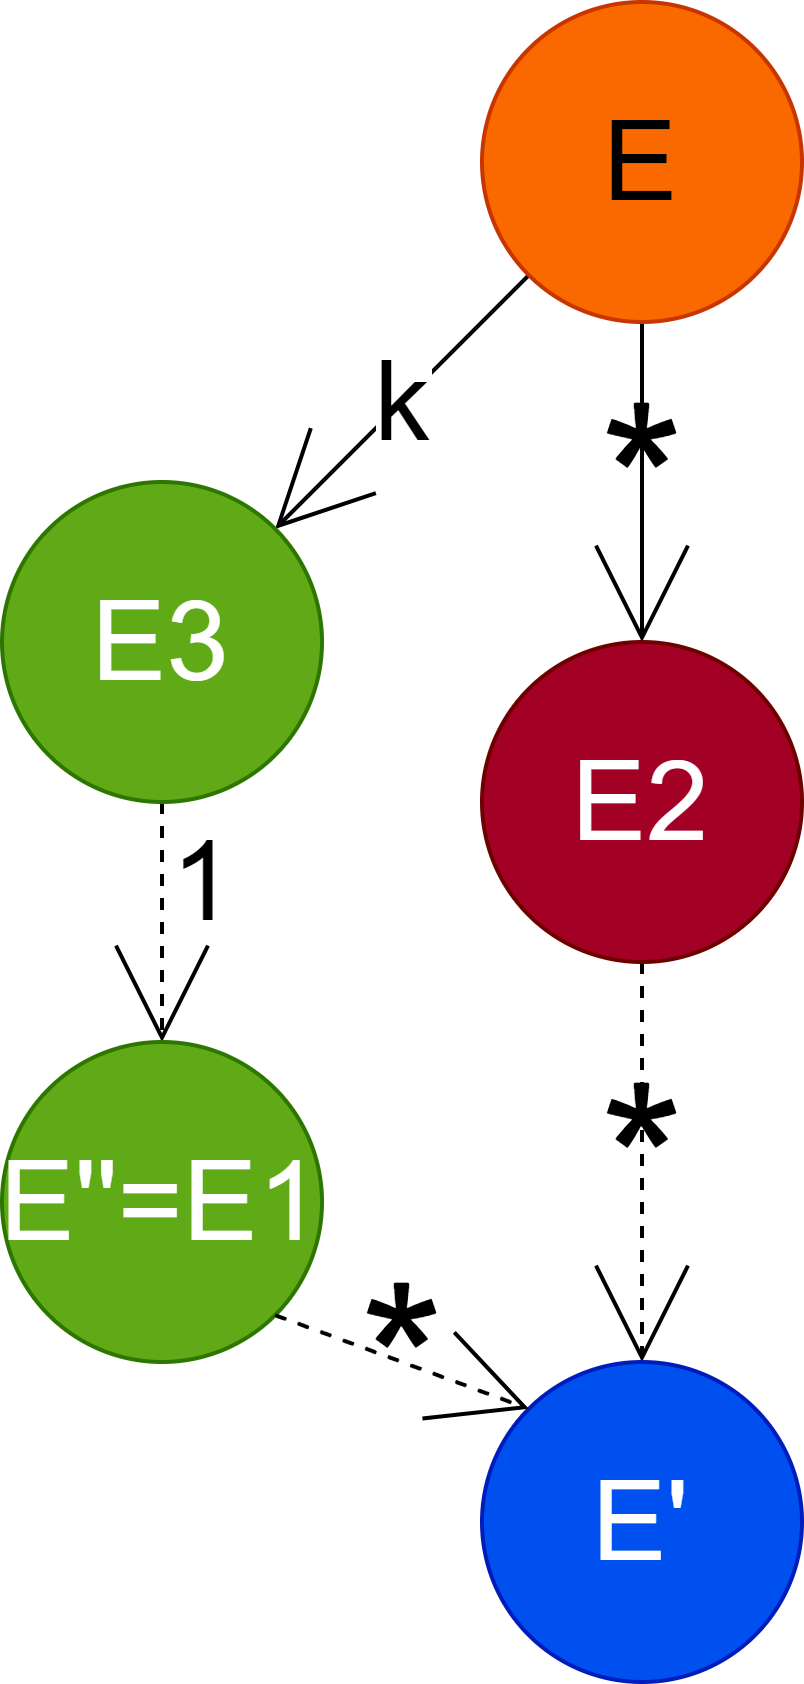
\includegraphics[scale=0.1]{confluence inductive case B.png}
                \end{center}
\end{document}
